\documentclass[11pt]{article}

\usepackage[margin=1in]{geometry}
\usepackage{amsmath, amssymb}
\usepackage{booktabs}
\usepackage{graphicx}
\usepackage{siunitx}
\usepackage{xcolor}
\usepackage[colorlinks=true, linkcolor=blue!60!black, urlcolor=blue!60!black]{hyperref}
\usepackage{enumitem}
\usepackage{tcolorbox}

\newtcolorbox{novicebox}[1][]{colback=blue!4, colframe=blue!40!black,
  title={For the newcomer: #1}, fonttitle=\bfseries}
\newtcolorbox{findingbox}[1][]{colback=orange!6, colframe=orange!60!black,
  title={V\&V finding: #1}, fonttitle=\bfseries}

\newcommand{\pu}{\,\text{pu}}
\newcommand{\dd}{\mathrm{d}}

\title{Verification and Validation of the DataCenter Gas-Plant and
  Turbine-Governor Models\\
  \large Equations, methods, and results --- written to be readable by a
  newcomer to power-system dynamics}
\author{DataCenter repository V\&V campaign}
\date{July 18, 2026}

\begin{document}
\maketitle

\begin{abstract}
This report documents the models implemented in the \texttt{DataCenter}
repository --- the IEEE PES-TR1 \textsc{GGOV1} and \textsc{TGOV1}
turbine-governor models, a two-mass gas-path model of the GE LM2500
aeroderivative gas turbine, a torsional shaft-fatigue model, and the
steady-state gas-plant thermodynamic surrogates --- together with the full
verification and validation (V\&V) campaign performed on them. Every
equation solved by the code is derived here from first principles, with
per-unit conventions spelled out, because unit-system mistakes were the
single largest class of defect found in the pre-V\&V code. Headline
results: the swing-equation + TGOV1 implementation matches the independent
ANDES simulator to \SI{0.124}{mHz}; the GGOV1 implementation reproduces the
Hannett \& Khan (1993) literature benchmark step response to 1.3\,\%; and a
Rowen-model reconstruction of the published Beluga~5 load-rejection event
matches the recorded speed trace with an RMS misfit of
$1.1\times10^{-3}\pu$. All 36 automated tests pass. A companion running log
(\texttt{docs/vv\_log.md}) records every change, and a constants dossier
(\texttt{docs/constants.md}) classifies every number in the models as
pinned, estimated, or placeholder.
\end{abstract}

\tableofcontents
\clearpage

%=====================================================================
\section{Introduction}
%=====================================================================

\subsection{What system are we modeling?}

The engineering question behind this repository: \emph{can a gas-turbine
power plant, disconnected from the bulk electric grid (``islanded''), keep
an AI data center alive?} AI training workloads swing their electrical
demand by large fractions in seconds. On the big interconnected grid those
swings are absorbed by thousands of machines; on an island with one or a
few gas turbines, every swing is a direct fight between the load and the
turbine's control system. The models here simulate that fight.

Three physical subsystems interact:
\begin{enumerate}[nosep]
  \item \textbf{The rotating machine.} A gas turbine spins a synchronous
    generator. The rotational kinetic energy stored in the shaft is the
    system's first line of defense: when load suddenly exceeds mechanical
    power, the shaft slows down and that kinetic energy covers the deficit
    for the first second or so. Shaft speed \emph{is} grid frequency, so
    ``the shaft slows down'' means ``the lights flicker at 59.5\,Hz.''
  \item \textbf{The governor.} A feedback controller that measures shaft
    speed and moves the fuel valve to restore it. The industry describes
    governors with standardized block diagrams --- \textsc{TGOV1} (simple)
    and \textsc{GGOV1} (detailed, gas-turbine-specific) from the IEEE PES
    Task Force report PES-TR1 (2013)~\cite{pestr1}. Using the standard
    models is what makes results communicable to grid engineers.
  \item \textbf{The thermodynamic plant.} Fuel in, electricity and hot
    exhaust out. Steady-state surrogate models convert operating points
    into fuel burn, efficiency, exhaust conditions, and CO$_2$.
\end{enumerate}

\subsection{What do ``verification'' and ``validation'' mean?}

\begin{novicebox}[V vs.\ V]
\textbf{Verification} asks: \emph{did we solve the equations right?} It
compares the code against mathematics --- analytic solutions, invariants
that must hold exactly (energy balances, steady-state identities), and
independent implementations of the same equations (here, the ANDES
simulator). \textbf{Validation} asks: \emph{did we solve the right
equations?} It compares the model against reality --- here, published field
tests on real gas turbines (Hannett \& Khan 1993) and published
thermodynamic data. A model can pass verification and fail validation (a
perfectly-solved wrong model) and vice versa.
\end{novicebox}

This campaign ran in phases: Phase~0 fixed defects found in a code review
(they are cataloged in Appendix~\ref{app:defects} --- read it; several are
instructive); Phase~1 verified; Phase~2 audited every constant; Phase~3
validated against literature; Phase~4 froze everything into an automated
regression suite (\texttt{pixi run vv-all}).

%=====================================================================
\section{Foundations: per-unit systems and the swing equation}
%=====================================================================

\subsection{The per-unit system}
\label{sec:pu}

Power-system engineers divide every quantity by a \emph{base} value and
work with the dimensionless ratios, called \emph{per-unit} (pu) values.

\begin{novicebox}[Why per-unit?]
If a generator is rated \SI{23}{MVA} and currently produces \SI{15}{MW},
its output is $15/23 = 0.652\pu$. The pu system makes machines of
different sizes directly comparable (``the valve is at 65\,\% of rating'')
and makes the equations cleaner. The catch --- and the source of the worst
bug found in this code --- is that \emph{a pu number is meaningless until
you know its base}. The same physical \SI{22}{MW} is $0.957\pu$ on a
\SI{23}{MVA} generator base but $1.000\pu$ on a \SI{22}{MW} turbine base.
\end{novicebox}

\paragraph{A worked example.} The LM2500 gen-set: $S_n = \SI{23}{MVA}$
(generator rating), $T_\text{rate} = \SI{22}{MW}$ (turbine rating). The
unit carries \SI{15}{MW}:
\[
  P_e^{(g)} = \frac{15}{23} = 0.652\pu \text{ (gen base)}, \qquad
  P_e^{(t)} = \frac{15}{22} = 0.682\pu \text{ (turbine base)}.
\]
The governor needs the turbine-base number (its fuel map is defined
against the turbine rating); the swing equation needs the gen-base number
(its inertia constant is defined against the MVA rating). The fuel valve
sits at $v = P_e^{(t)}/K_{turb} + W_{fnl} = 0.682/1.5 + 0.2 = 0.655\pu$
stroke --- note this is a \emph{third} normalized quantity (fuel-flow
units), numerically close to the power numbers only by coincidence of
$K_{turb}$ and $W_{fnl}$. Defect G2 (Appendix~\ref{app:defects}) happened
precisely because a fuel-stroke number was passed somewhere a power
fraction was expected.

Two bases coexist in this repository, deliberately:
\begin{itemize}[nosep]
  \item \textbf{Generator base} $S_n$ = \SI{23}{MVA}: used by the swing
    equation (rotor mechanics), because machine inertia data is quoted on
    it.
  \item \textbf{Turbine base} $T_\text{rate}$ = \SI{22}{MW}: used by
    \emph{everything inside the governor} (valve stroke, fuel flow,
    mechanical power, limits), because IEEE PES-TR1 \S3.3 defines the
    GGOV1 parameters on it (PSS/E calls this base \texttt{Trate}).
\end{itemize}
The single conversion constant is
\begin{equation}
  k_b \;=\; \frac{T_\text{rate}}{S_n} \;=\; \frac{22}{23} \;=\; 0.9565,
  \qquad
  P^{\text{(gen base)}} = k_b \, P^{\text{(turbine base)}} .
  \label{eq:kb}
\end{equation}
It is applied at exactly two places: mechanical power entering the swing
equation, and electrical power entering the governor's power transducer.
Appendix~\ref{app:defects} (defect G1) describes what went wrong when the
pre-V\&V code tried to blend the two bases by hand-editing one limit.

\subsection{The swing equation}
\label{sec:swing}

Newton's second law for a rotating shaft with moment of inertia $J$
(\si{kg.m^2}), mechanical drive torque $\tau_m$ and electrical braking
torque $\tau_e$ (\si{N.m}):
\begin{equation}
  J \,\frac{\dd \Omega}{\dd t} \;=\; \tau_m - \tau_e ,
\end{equation}
where $\Omega$ is the mechanical angular speed (\si{rad/s}). Define the
\emph{inertia constant}
\begin{equation}
  H \;=\; \frac{\tfrac12 J \Omega_0^2}{S_n}
  \qquad \text{(units: seconds),}
  \label{eq:H}
\end{equation}
the kinetic energy at rated speed divided by the machine rating. $H$
answers: \emph{for how many seconds could the stored kinetic energy alone
supply rated power?} Aeroderivative gen-sets are light: $H \approx
1.5$--$3.5$\,s. Normalizing speed as $\omega = \Omega/\Omega_0$ and power
by $S_n$, and using $P = \tau\,\Omega$, the equation becomes (to first
order near $\omega = 1$) the standard \emph{swing equation}:
\begin{equation}
  \boxed{\;2H \,\frac{\dd\omega}{\dd t} \;=\; P_m - P_e - D(\omega - 1)\;}
  \qquad
  \frac{\dd\delta}{\dd t} = \omega_0(\omega - 1),
  \label{eq:swing}
\end{equation}
with $\omega_0 = 2\pi\cdot 60$\,\si{rad/s}, rotor electrical angle
$\delta$, and damping coefficient $D$. This ``power form'' ($P_m - P_e$
rather than the strict torque form $(P_m - P_e)/\omega$) was verified in
Phase~1 to be \emph{exactly} what the ANDES simulator solves: ANDES's
classical machine uses the standard speed-voltage approximation (stator
flux evaluated at $\omega = 1$), under which electrical torque equals
electrical power, and its governor output enters the torque equation
one-to-one (\S\ref{sec:andescross}).

\begin{novicebox}[Frequency, speed, and why 60\,Hz]
The generator here has 2 magnetic poles, so electrical frequency equals
shaft speed: \SI{3600}{rpm} $=$ \SI{60}{rev/s} $=$ \SI{60}{Hz}. When
$\omega = 0.99\pu$, the grid is at \SI{59.4}{Hz}. Data-center power
supplies and the turbine itself have under/over-frequency protection, so
excursions of a few hundred mHz matter and excursions of a few Hz trip
equipment.
\end{novicebox}

\subsection{Load damping}

Real loads draw slightly less power when frequency drops (motors slow
down, etc.). This is modeled on the load, not the machine:
\begin{equation}
  P_e(t,\omega) \;=\; P_\text{demand}(t)\,\bigl[1 + \alpha(\omega - 1)\bigr],
  \qquad \alpha = 1.5,
  \label{eq:loaddamp}
\end{equation}
with $\alpha$ in Kundur's typical range 1--2~\cite{kundur}. Because the
load damping is explicit, the machine damping is set to $D = 0$: the
pre-V\&V code carried \emph{both} $D = 1$ and $\alpha = 1.5$, double
counting the same physics and making every predicted frequency dip
optimistic (defect G5).

\subsection{Droop: how multiple governors share load}
\label{sec:droop}

A governor could hold frequency exactly at 60\,Hz (\emph{isochronous}
control), but two isochronous governors on one grid fight each other.
The standard solution is \emph{droop}: the governor deliberately lets
steady-state frequency fall linearly with its power output,
\begin{equation}
  \Delta\omega_{ss} \;=\; -R\,\Delta P_{ss},
  \qquad R = 0.04 \;(4\,\%),
  \label{eq:droop}
\end{equation}
i.e., going from no load to full load lowers the machine's steady
frequency target by 4\,\% (2.4\,Hz), so machines share load in proportion
to their ratings without communicating. For a \emph{single} islanded unit,
isochronous control (or droop plus a slow secondary loop) is standard
practice; the implementation supports both (\texttt{rselect} parameter,
\S\ref{sec:ggov1speed}), and the droop identity \eqref{eq:droop} is one of
the exact tests in the verification suite.

%=====================================================================
\section{The TGOV1 governor model (legacy, Tier A)}
%=====================================================================
\label{sec:tgov1}

\textsc{TGOV1} is the simplest standard turbine-governor model: one lag,
one lead-lag, one droop gain. In this project it is the \emph{legacy}
model (kept because it is what ANDES can cross-simulate and it anchors the
project's history); GGOV1 is the reference model. The block structure, now
implemented exactly per the standard:
\begin{equation}
  \underbrace{\frac{1}{R}\bigl(\Delta\omega_\text{ref} - \Delta\omega\bigr) + P_\text{ref}}_{\text{droop input}}
  \;\longrightarrow\;
  \underbrace{\frac{1}{1 + sT_1}}_{\substack{\text{valve servo,}\\ \text{non-windup } [V^{min},\,V^{max}]}}
  \;\longrightarrow\;
  \underbrace{\frac{1 + sT_2}{1 + sT_3}}_{\text{turbine lead-lag}}
  \;\longrightarrow\; P_m - D_t\,\Delta\omega .
  \label{eq:tgov1}
\end{equation}

\begin{novicebox}[Reading transfer-function blocks]
$\frac{1}{1+sT}$ is a \emph{first-order lag}: the output chases the input
with time constant $T$ (63\,\% of a step change after $T$ seconds). In
state-space form, $\dot{x} = (u - x)/T$. The lead-lag
$\frac{1+sT_2}{1+sT_3}$ responds immediately with a fraction $T_2/T_3$ of
a step and then relaxes to the full value with time constant $T_3$ --- it
models the fact that some turbine power responds quickly to the valve and
the rest waits for the gas path to fill.
\end{novicebox}

The ODE system solved (state vector $[\delta, \omega, v, x_2,
P_\text{fuel}]$, all pu on the \emph{generator} base --- valid for TGOV1
because its implicit turbine gain is 1, so valve pu $=$ power pu):
\begin{align}
  \dot v &= \frac{1}{T_1}\Bigl[P_\text{ref} + \tfrac{1-\omega}{R} - v\Bigr]
     \quad\text{(zeroed if it would push $v$ past } V^{min}\!/V^{max}\text{)},\\
  \dot x_2 &= \frac{v - x_2}{T_3}, \qquad
  P_m = x_2 + \frac{T_2}{T_3}(v - x_2) - D_t(\omega - 1), \\
  2H\dot\omega &= P_m - P_e(t,\omega), \qquad
  \dot P_\text{fuel} = \frac{v - P_\text{fuel}}{T_\text{comb}} .
\end{align}
Parameters: $R=0.04$, $T_1 = 0.15$\,s, $T_2 = 0.3$\,s, $T_3 = 1.5$\,s,
$V^{max} = 22/23$ (the turbine rating on the generator base --- correct
\emph{here} because valve pu $=$ power pu), $V^{min} = 0.15$.

\begin{findingbox}[slew limits inside a tight loop cause limit cycles]
The pre-V\&V code added a $\pm0.1\pu/\text{s}$ valve rate limit. Placed at
the \emph{standard} limiter location (on the valve state, inside the droop
loop), this produces a sustained $\pm1.3$\,Hz oscillation at LM2500 gains:
the loop gain is $1/(R\,T_1) \approx 167\,\text{s}^{-1}$, the commanded
slew hugely exceeds the limit during transients, and the resulting phase
lag destabilizes the loop --- a classic describing-function instability,
not a numerical artifact. (The old code ``worked'' only because its rate
limiter sat outside the feedback path, a nonstandard structure that also
added a spurious second pole at $1/T_1$.) Standard TGOV1 has no rate
limit; rate-limited fuel dynamics belong in GGOV1, whose $\pm0.05$ error
clamp bounds the commanded rate. The option is now off by default.
\end{findingbox}

%=====================================================================
\section{The GGOV1 governor model (reference, Tier B)}
%=====================================================================
\label{sec:ggov1}

\textsc{GGOV1} (PES-TR1 Fig.~3-5) is the industry-standard gas-turbine
governor model. It captures the three control loops every modern GT
control system (GE Speedtronic, Woodward) actually runs, arbitrated by a
\emph{low value select} (LVS): whichever controller asks for the
\emph{least} fuel wins.

\subsection{State vector and parameters}

The implementation integrates twelve states:

\begin{table}[h]\centering
\small
\begin{tabular}{llll}
\toprule
state & meaning & base & equation \\
\midrule
$\delta$ & rotor electrical angle (rad) & --- & $\dot\delta = \omega_0(\omega-1)$ \\
$\omega$ & rotor speed & pu of $2\pi 60$ & swing eq.\ \eqref{eq:swing} \\
$\tilde P_e$ & measured electrical power & turbine & $T_{pelec}$ lag \\
$x_i$ & speed-PI integrator & turbine & \eqref{eq:backcalc} \\
$x_{ka}$ & acceleration integrator ($= f_{sra}$) & turbine & \eqref{eq:backcalc} \\
$x_a$ & speed lag for the $\dd\omega/\dd t$ filter & pu & $T_a$ lag \\
$x_{iT}$ & temperature-PI integrator & turbine & \eqref{eq:backcalc} \\
$x_{tload}$ & temperature-signal lag & turbine & $T_{fload}$ lag \\
$x_{tsab}$ & temperature-signal lead-lag state & turbine & $T_{sa}/T_{sb}$ \\
$v$ & fuel-valve stroke & turbine & actuator + limits \\
$x_t$ & turbine lead-lag state & turbine & $T_b/T_c$ on $W_f$ \\
$P_\text{fuel}$ & combustor-lagged fuel signal & turbine & $T_\text{comb}$ lag \\
\bottomrule
\end{tabular}
\caption{GGOV1 state vector as implemented
(\texttt{gas\_plant/dynamics/ggov1.py}).}
\end{table}

\begin{table}[h]\centering
\small
\begin{tabular}{llll@{\qquad}llll}
\toprule
param & value & unit & status & param & value & unit & status \\
\midrule
$R$ & 0.04 & pu & P & $K_{turb}$ & 1.5 & --- & P \\
$T_{pelec}$ & 1.0 & s & P & $W_{fnl}$ & 0.2 & pu & P \\
Max/MinERR & $\pm$0.05 & pu & P & $T_b$, $T_c$ & 0.1, 0 & s & P \\
$K_{pgov}$ & 10 & --- & P$^{*}$ & $V^{max}$, $V^{min}$ & 1.0, 0.15 & pu & P \\
$K_{igov}$ & 2 & --- & P$^{*}$ & $R_{open/close}$ & $\pm$0.10 & pu/s & P \\
$a_\text{set}$ & 0.01 & pu/s & P & $L_{dref}$ & 1.0 & pu(t) & P \\
$K_a$, $T_a$ & 10, 0.1 & ---, s & P & $K_{pload}$, $K_{iload}$ & 2, 0.67 & --- & P \\
$T_{act}$ & 0.15 & s & E & $T_{fload}$, $T_{sa}$, $T_{sb}$ & 3, 4, 5 & s & P \\
$H$ & 2.8 & s & \textbf{PL} & $D_m$ & 0 & --- & P \\
$\alpha$ & 1.5 & --- & P(range) & $\eta_\text{design}$ & 0.365 & --- & E \\
\bottomrule
\end{tabular}
\caption{Parameter values with dossier status: P = pinned (PES-TR1
Appendix C unless noted), E = estimated, PL = placeholder.
$^{*}$pinned to the \emph{generic} PES-TR1 value; flagged for vendor
retune (Hannett's field-derived governors are 2--4$\times$ hotter).
Full provenance per row in \texttt{docs/constants.md}.}
\end{table}

\subsection{Per-unit convention}
All governor signals below --- valve stroke $v$, fuel flow $W_f$, the
controller outputs $f_{srn}, f_{sra}, f_{srt}$, mechanical power
$P_m^{(t)}$, and the limits --- are pu on the \emph{turbine base}
$T_\text{rate} = \SI{22}{MW}$. The swing equation stays on the generator
base; the conversion \eqref{eq:kb} appears exactly twice:
\begin{equation}
  2H\,\dot\omega = k_b\,P_m^{(t)} - P_e^{(g)} - D(\omega-1),
  \qquad
  P_e^{(t)} = P_e^{(g)}/k_b .
\end{equation}

\subsection{Loop 1: speed/power governor}
\label{sec:ggov1speed}

A PI controller on a speed error that includes selectable droop feedback:
\begin{equation}
  e_s =
  \begin{cases}
    (1-\omega) + R\,(P_\text{ref} - \tilde P_e) & \texttt{rselect}=1
      \ \text{(droop on electrical power; default)}\\[2pt]
    (1-\omega) & \texttt{rselect}=0 \ \text{(isochronous)}\\[2pt]
    (1-\omega) + R\,(P_\text{ref} - v) & \texttt{rselect}=-1
      \ \text{(droop on valve stroke)}\\[2pt]
    \dfrac{(1-\omega) + R\,(P_\text{ref} - x_{i})}{1 + R\,K_{p}} &
      \texttt{rselect}=-2 \ \text{(droop on governor output)}
  \end{cases}
  \label{eq:rselect}
\end{equation}
clamped to $[\text{MinERR}, \text{MaxERR}] = [-0.05, +0.05]$, then
\begin{equation}
  f_{srn} = K_{pgov}\, e_s + x_{i},
  \qquad \dot x_{i} = K_{igov}\,e_s \;-\; \text{(anti-windup, \S\ref{sec:aw})}.
\end{equation}
Here $\tilde P_e$ is the electrical power measured through a transducer
lag $\dot{\tilde P_e} = (P_e^{(t)} - \tilde P_e)/T_{pelec}$. The
\texttt{rselect}$=-2$ case contains an algebraic loop ($e_s$ depends on
$f_{srn}$ which depends on $e_s$); it is solved in closed form as shown.
The pre-V\&V code documented four \texttt{rselect} modes but implemented
only one --- notably missing isochronous, the natural mode for a single
islanded unit (defect G4).

\subsection{Loop 2: acceleration limiter}
The rotor acceleration is estimated with a washout filter (the exact
state-space realization of $s/(1+sT_a)$):
\begin{equation}
  \dot x_a = \frac{\omega - x_a}{T_a}, \qquad
  \hat a = \frac{\omega - x_a}{T_a}, \qquad
  e_a = a_\text{set} - \hat a, \qquad
  f_{sra} = x_{ka}, \quad \dot x_{ka} = K_a e_a - \text{(a.w.)}
\end{equation}
It only takes over when the shaft accelerates faster than $a_\text{set} =
0.01\pu/\text{s}$ (startup, load rejection).

\subsection{Loop 3: temperature (thermal) limiter}
Gas turbines are power-limited by hot-section temperature. GGOV1 proxies
exhaust temperature by fuel flow: $W_f$ passes through a lead-lag
$(1+sT_{sa})/(1+sT_{sb})$ (thermocouple/radiation-shield dynamics) and a
lag $1/(1+sT_{fload})$, giving $x_{tload}$; the limiter then runs a PI on
\begin{equation}
  e_T = \underbrace{\Bigl(\frac{L_{dref}}{K_{turb}} + W_{fnl}\Bigr)}_{t_{lim}
   \;=\; \text{fuel flow at the thermal limit}} - \; x_{tload},
  \qquad
  f_{srt} = K_{pload}\,e_T + x_{iT}, \quad \dot x_{iT} = K_{iload}e_T - \text{(a.w.)}
\end{equation}
With $L_{dref} = 1.0$ on the turbine base, the limiter caps continuous
output at exactly $1.0\pu \times \SI{22}{MW} = \SI{22}{MW}$ --- this is
\emph{the} enforcement of the turbine's thermal rating (verified by test:
a \SI{25}{MW} demand settles at $P_m = \SI{22.000}{MW}$ with the
temperature limiter selected). The pre-V\&V code, with its mixed bases,
enforced 23\,MW here and 26.1\,MW at the valve limit while claiming 22\,MW
(defect G1).

\subsection{Low value select and anti-windup}
\label{sec:aw}

\begin{equation}
  f_{sr} = \min\left(f_{srn},\, f_{sra},\, f_{srt}\right).
\end{equation}

\begin{novicebox}[Integrator windup]
A PI controller's integrator keeps accumulating error even while its
output is being ignored (not selected by the LVS, or the valve is pinned
at a limit). When conditions change, the wound-up integrator forces a
long, sluggish overshoot before the controller re-engages. Every
practical multi-loop controller needs \emph{anti-windup}.
\end{novicebox}

This implementation uses an always-active \emph{back-calculation} form on
all three integrators:
\begin{equation}
  \dot x_{i} = K_i\,e \;-\; K_{bc}\,\bigl(f_{srX} - f_{sr}\bigr).
  \label{eq:backcalc}
\end{equation}
Because $f_{sr}$ is the minimum, $(f_{srX} - f_{sr}) \ge 0$ always: it is
\emph{zero} for the selected controller (pure PI, no distortion) and
positive for unselected ones, pulling their integrators down to track the
actual command so they re-engage cleanly. The form is continuous (no
if/else switching), which keeps the ODE solver's step size healthy. The
tracking gain $K_{bc}$ is an implementation knob, not physics; Phase~1
verified that varying it over a $25\times$ range moves a step-response
nadir by only 2.1\,mHz.

\subsection{Valve actuator and turbine}
\begin{align}
  \dot v &= \text{clip}\!\left(\frac{\text{clip}(f_{sr},V^{min},V^{max}) - v}{T_{act}},\;
      R_{close},\, R_{open}\right)
      \quad\text{(zeroed at the position limits)},\\
  W_f &= v\cdot\omega^{\,[\texttt{flag}=1]} \cdot \omega^{D_m[D_m<0]}, \qquad
  \dot x_t = \frac{W_f - x_t}{T_b},\\
  P_m^{(t)} &= K_{turb}\Bigl(x_t + T_c\dot x_t - W_{fnl}\Bigr)
    \;-\; D_m(\omega-1)\,[D_m>0].
  \label{eq:turbine}
\end{align}
Two constants deserve explanation for the newcomer:
\begin{itemize}[nosep]
\item $W_{fnl} = 0.2$ is the \emph{full-speed no-load} fuel: a spinning,
  unloaded gas turbine still burns $\sim$20\,\% of rated fuel just to
  drive its own compressor. Power is proportional to fuel \emph{above}
  that floor --- hence $P_m = K_{turb}(W_f - W_{fnl})$ with $K_{turb} =
  1.5 \approx 1/(1 - W_{fnl}\cdot\ldots)$ chosen so $W_f = 0.867$ gives
  rated power.
\item $V^{max} = 1.0$ is a valve \emph{stroke} limit, not a power limit.
  At the stroke limit the turbine could transiently make
  $K_{turb}(1.0-0.2) = 1.2\pu = \SI{26.4}{MW}$ --- short-term capability
  that the temperature limiter then winds back to \SI{22}{MW} over its
  $T_{fload}$/PI time scale. Both ceilings are now explicit, tested
  properties.
\item $D_m$: for $D_m > 0$ the term \emph{subtracts} power as speed rises
  (damping). The pre-V\&V code had the sign flipped --- energy injection
  on overspeed (defect G3); the test suite now pins the direction
  (a load rejection peaks at \SI{75.1}{Hz} with $D_m{=}0$ vs
  \SI{72.0}{Hz} with $D_m{=}0.5$).
\end{itemize}

\subsection{Steady-state initialization}
\label{sec:ic}
Transient studies must start from an exact equilibrium or the first
seconds of every run are polluted by artificial settling. Setting all
derivatives to zero at $\omega=1$, load $P_{e0}^{(t)}$:
\begin{equation}
  v_0 = \frac{P_{e0}^{(t)}}{K_{turb}} + W_{fnl}, \qquad
  x_{i,0} = f_{sr,0} = v_0, \qquad
  x_{ka,0} = v_0 + \frac{K_a a_\text{set}}{K_{bc,a}}, \qquad
  x_{iT,0} = v_0 + \frac{K_{iload}e_{T0}}{K_{bc,T}} - K_{pload}\,e_{T0},
\end{equation}
where the small offsets come from balancing the back-calculation terms
\eqref{eq:backcalc} of the \emph{unselected} loops. Phase~1 verified
$\lVert\text{RHS}\rVert < 3\times10^{-15}$ at five operating points ---
the initial condition is an equilibrium to machine precision.

\subsection{Fuel accounting}
\label{sec:fuel}
Fuel mass flow is computed \emph{natively} from the governor's own fuel
signal:
\begin{equation}
  \dot P_\text{fuel} = \frac{W_f - P_\text{fuel}}{T_\text{comb}},
  \qquad
  \dot m_\text{fuel} = w_\text{base}\, P_\text{fuel},
  \qquad
  w_\text{base} = \frac{T_\text{rate}}{\eta_\text{design}\, \text{LHV} \,
      \bigl(\tfrac{L_{dref}}{K_{turb}} + W_{fnl}\bigr)} = \SI{1.419}{kg/s}\ \text{per pu},
\end{equation}
anchored so that rated output burns $22\,\text{MW}/(0.365 \times
49\,\text{MJ/kg}) = \SI{1.230}{kg/s}$ ($\eta_\text{design} = 0.365$,
status \textsc{estimated} --- see the constants dossier; cross-checked
against the NAVEDTRA figure of 9{,}000\,lb/h at 26{,}250 shaft hp
$\Rightarrow$ 35.3\,\% shaft efficiency). The pre-V\&V code instead fed
the raw \emph{valve stroke} into a surrogate expecting a \emph{power
fraction}, double-counting no-load fuel (defect G2) --- every prior fuel
total was biased by it.

%=====================================================================
\section{Two-mass gas-path model (Tier C)}
%=====================================================================
\label{sec:multishaft}

The LM2500 is a \emph{two-spool} engine: the gas-generator spool (HP
compressor + HP turbine, $\sim$9{,}500\,rpm at full power) is connected to
the power-turbine/generator spool (3{,}600\,rpm) \emph{only by flowing
gas}, not by a shaft. When the fuel valve opens, the gas generator must
spool up before extra power reaches the generator --- a lag invisible to
single-mass models. The two-mass model:
\begin{align}
  2H_{hp}\,\dot\omega_{hp} &= P_m^{(t)} - P_c, \qquad
  P_c = \max\bigl[0,\; K_c\,(\omega_{hp} - \omega_{hp}^\text{idle})\bigr],\\
  2H_{pt}\,\dot\omega_{pt} &= k_b P_c - P_e^{(g)} - D_{pt}(\omega_{pt}-1),
\end{align}
with $\omega_{hp}^\text{idle} = 4900/9500 = 0.516$ (pinned to the LM2500
Pocket Guide) and $K_c = 1/(1-\omega_{hp}^\text{idle})$ normalized so full
NGG speed delivers rated power. The governor's speed input is
$\omega_{pt}$ (the speed pickups are on the power-turbine shaft).

\textbf{Honesty box:} the linear coupling law $P_c(\omega_{hp})$ is a
\textsc{placeholder}. Real free-turbine power vs.\ gas-generator speed is
strongly nonlinear ($\sim$cubic) and depends on PT speed; the implied
spool time constant $2H_{hp}/K_c \approx \SI{0.29}{s}$ vs.\ a real NGG's
0.5--1.5\,s. Tier~C transient \emph{deltas} (e.g.\ ``the nadir is deeper
than single-mass models predict'') are qualitative until this is
calibrated against a recorded spool-up trace. The verification suite still
holds the model to exact invariants: the steady NGG-speed-to-load map, an
HP-rotor energy balance $2H_{hp}\Delta\omega_{hp} = \int (P_m^{(t)} -
P_c)\,\dd t$ to $10^{-3}$, and equilibrium initialization. (A former
\texttt{delta\_hp} ``angle'' state, which drifted secularly because the HP
spool has no meaningful electrical angle, was removed --- caught by the
equilibrium test.)

%=====================================================================
\section{Torsional shaft and fatigue model (Tier E)}
%=====================================================================
\label{sec:torsional}

The one \emph{physical} shaft in the machine --- the coupling between the
power turbine and the generator rotor --- twists elastically and has a
torsional resonance. Load steps ring it; the ringing consumes fatigue
life.

\subsection{Dynamics, and a per-unit derivation worth reading}
Two masses ($M = 2H$) joined by a torsional spring $k$ and damper $c$,
tracked in \emph{differential} coordinates
($\theta$ = twist angle, $\omega_d$ = speed difference; the common-mode
speed is imposed from the Tier~C solution so it cannot drift):
\begin{equation}
  \dot\theta = \omega_0\,\omega_d, \qquad
  \dot\omega_d = \frac{\tau_{pt}}{M_{pt}} + \frac{\tau_{e}}{M_{gen}}
   - \frac{T_\text{shaft}}{I_r}, \qquad
  T_\text{shaft} = k\,\theta + c\,\omega_d, \qquad
  I_r = \frac{M_{pt} M_{gen}}{M_{pt}+M_{gen}} .
\end{equation}
Combining gives $\ddot\theta = -\,(\omega_0 k / I_r)\,\theta + \ldots$, so
the natural frequency is
\begin{equation}
  \boxed{\;\omega_n = \sqrt{\frac{\omega_0\,k}{I_r}}
  \quad\Longrightarrow\quad
  k = \frac{\omega_n^2 I_r}{\omega_0}\;}
  \label{eq:kpu}
\end{equation}
Note the factor $\omega_0 = 377$\,rad/s that appears because pu speed
multiplies $\omega_0$ in the angle equation but the inertia equation is
already normalized. The repository's own history makes the point: an
earlier version omitted it, silently making the ``22\,Hz'' mode actually
427\,Hz. \emph{Per-unit derivations must be done, not assumed.} The
identity \eqref{eq:kpu} is now pinned by a test ($f_n = 22.0000$\,Hz).

\subsection{From torque history to fatigue damage}
\begin{enumerate}[nosep]
\item \textbf{Stress:} $\tau = T/W_t$ with the polar section modulus of a
  hollow shaft $W_t = \tfrac{\pi}{16}\,(D^4 - d^4)/D$.
\item \textbf{Detrend:} \texttt{detrend\_rolling\_median} separates slow
  operating-point shifts (low-cycle events, counted separately) from the
  oscillations that rainflow should count --- rainflow on a non-stationary
  signal buries the oscillation cycles under the trend.
\item \textbf{Rainflow} (ASTM E1049 4-point method) reduces the stress
  history to cycles with amplitude $S_a$ and mean $S_m$.
  \begin{novicebox}[what rainflow counting does]
  Fatigue damage is caused by closed stress--strain hysteresis loops, not
  by the raw wiggles of the signal. Rainflow finds those loops: reduce the
  signal to its turning points; then, scanning a stack of the last three
  turning points, whenever the middle excursion is smaller than or equal
  to the one that follows it, that middle excursion is a closed cycle ---
  extract it (range = its height, mean = its midpoint) and continue.
  Leftover half-cycles at the end count with weight $\tfrac12$. The result
  is a histogram of (amplitude, mean) pairs that the S--N curve can
  consume. Rainflow assumes a roughly stationary signal --- hence the
  detrending step before it.
  \end{novicebox}
\item \textbf{Goodman correction} penalizes cycles riding on a mean
  stress: $S_a^{eq} = S_a / (1 - S_m/S_{u,\text{shear}})$,
  $S_{u,\text{shear}} = 0.6\,S_u$.
\item \textbf{Basquin S--N + Miner's rule:}
  $N_f = N_\text{ref}\,(S_{a,\text{ref}}/S_a^{eq})^{m}$ and damage $D =
  \sum n_i/N_{f,i}$; failure at $D = 1$.
\end{enumerate}
All material and geometry numbers are \textsc{placeholder}-class (typical
AISI 4340, invented shaft dimensions, assumed 22\,Hz mode): the model is a
duty-cycle \emph{screening} tool. Its screening conclusion stands:
Load17-class demand profiles (3\,s cadence) are far too slow to excite the
torsional mode --- shaft fatigue risk comes from faults, motor starts, and
breaker events, not AI load-following.

%=====================================================================
\section{Gas-plant thermodynamic models}
%=====================================================================
\label{sec:thermo}

\subsection{Willans line: part-load fuel and efficiency}
For dispatch purposes a gas turbine is well described by the
\emph{Willans line} --- fuel flow affine in load:
\begin{equation}
  \dot m_f(L) = \dot m_{f,\text{rated}}\bigl[b + (1-b)L\bigr]
  \quad\Longrightarrow\quad
  \eta(L) = \eta_\text{fl}\,\frac{L}{b + (1-b)L},
  \label{eq:willans}
\end{equation}
with no-load fuel fraction $b = 0.2$ (deliberately the same number as
GGOV1's $W_{fnl}$). For the LM9000 ($\eta_\text{fl} = 0.3952$) this gives
32.9\,\% at half load and 22.0\,\% at 20\,\% load --- consistent with real
aeroderivative behavior and with the ThermoPower surrogate's shape. It
replaced a quadratic that claimed 39.0\,\% at half load (defect P1;
physically impossible for a machine with idle losses).

\subsection{Combined cycle energy balance}
The bottoming cycle recovers exhaust heat:
\begin{equation}
  Q_\text{HRSG} = \dot m_\text{exh}\, c_p\,
     \max(T_\text{exh} - T_\text{stack}, 0), \qquad
  P_{st} = \eta_b \, Q_\text{HRSG}, \qquad
  \eta_b = \eta_{b,\text{nom}}\,
     \frac{T_\text{exh}-T_\text{stack}}{T_\text{exh,nom}-T_\text{stack}} .
\end{equation}
The linear derate of $\eta_b$ with exhaust temperature is a pragmatic fit
form (an earlier claim that it came from PES-TR1/CIGRE-238 was wrong and
is retracted in the code). For the LM9000 CC, $\eta_{b,\text{nom}}$ is
\emph{auto-tuned} so the design point hits the datasheet 72.471\,MW
exactly (solution: 0.288); fuel, power, and CO$_2$ then all remain
physical with no post-hoc rescaling.

\subsection{CO$_2$ accounting}
$\dot m_{CO_2} = f \cdot \dot m_\text{fuel}$ with $f = 2.75$
(stoichiometric CH$_4$, $44.009/16.043$) for generic natural gas and $f =
2.65$ for the LM9000 (back-calculated from its datasheet 492.9\,kg/MWh;
the EPA pipeline-gas factor converts to $\approx 2.63$\,kg/kg ---
consistent).

%=====================================================================
\section{The Rowen/Hannett model (for validation only)}
%=====================================================================
\label{sec:rowen}

To compare against the 1993 field-test literature on its own terms, the
Rowen (1983) simplified gas-turbine model, in Hannett \& Khan's
parameterization, was implemented:
\begin{equation}
  e = \omega_\text{ref}-\omega
  \;\rightarrow\;
  \underbrace{\frac{W(Xs+1)}{Ys+Z}}_{\text{governor}}
  \;\rightarrow\; \text{clip}
  \;\rightarrow\;
  \underbrace{\frac{a}{bs+c}}_{\text{valve positioner}}
  \;\rightarrow\;
  \underbrace{\frac{1}{t_f s+1}}_{\text{fuel system}}
  \;\rightarrow\; W_f
\end{equation}
\begin{equation}
  W_f' = (K_3 V_{ce} + K_6)\,\omega \quad (K_6 = 1-K_3), \qquad
  \text{lag } T_{CD}, \qquad
  f_2 = a_{f2} + b_{f2}W_f + c_{f2}(1-\omega), \qquad
  P_m = f_2\,\omega .
\end{equation}
Droop $= Z/W$. The ``Typical Gas'' torque law is $f_2 = 1.3\,W_f - 0.299 +
0.5(1-\omega)$, which satisfies the steady-state identity $f_2(W_f{=}1,
\omega{=}1) = 1$ (the coefficients encode the same no-load-fuel physics as
GGOV1's $K_{turb}, W_{fnl}$: $b_{f2}K_3 \approx 1$, $a_{f2} + b_{f2}K_6
\approx 0$). The temperature loop is omitted: the paper states it sits at
its maximum limit throughout these tests. The vendored table's ``Typical
Gas'' $c_{f2} = 1.5$ is treated as a transcription artifact (Rowen 1983
and every field-derived unit row use 0.5).

%=====================================================================
\section{Verification results (Phase 1)}
%=====================================================================
\label{sec:verification}

\subsection{Cross-simulation against ANDES}
\label{sec:andescross}

The strongest verification available: run \emph{the same} single-machine
islanded scenario (GENCLS $H{=}2.8$\,s, TGOV1 $R{=}0.04$,
$T_{1,2,3}{=}0.15/0.3/1.5$\,s, constant-power load stepped
15$\rightarrow$18\,MW) in this repository's scipy code and in ANDES 2.0
(an independently developed, symbolically-compiled DAE simulator), and
compare trajectories point-by-point.

\begin{table}[h]\centering
\begin{tabular}{lcc}
\toprule
 & ANDES 2.0 & scipy (this repo) \\
\midrule
frequency nadir & 59.2326\,Hz & 59.2326\,Hz \\
final frequency & 59.6870\,Hz & 59.6870\,Hz \\
max $|\Delta\omega|$ over 30\,s & \multicolumn{2}{c}{$\mathbf{0.124}$\,\textbf{mHz}} \\
max $|\Delta P_m|$ & \multicolumn{2}{c}{$8.6\times10^{-5}\pu$ (2\,kW)} \\
\bottomrule
\end{tabular}
\caption{TGOV1 cross-simulation (\texttt{pixi run vv-crosscheck}).
Agreement is at solver tolerance.}
\end{table}

Reaching this agreement required (and therefore documented) three facts
about ANDES that were previously assumptions: (i) a single-bus case leaves
the machine's network equations degenerate (frequency frozen) --- a two-bus
case is required; (ii) the comparison line must be lossless, since a
$33$\,kW $I^2r$ loss shows up as a 3.4\,mHz steady-state offset; (iii)
ANDES's classical machine uses the speed-voltage approximation, under
which its swing equation \emph{is} the power form \eqref{eq:swing}, and
its governor output enters the torque equation one-to-one --- verified in
the ANDES source (GENBase/GENCLS), not guessed. ANDES has no GGOV1 model,
so GGOV1 is verified by the analytic methods below instead (a documented
deviation from the plan).

\subsection{Small-signal verification of GGOV1}
At operating points 5, 11.5, 15, 20, and 21.9\,MW
(\texttt{pixi run vv-smallsignal}):
\begin{itemize}[nosep]
\item \textbf{Equilibrium:} $\lVert \text{RHS} \rVert_\infty <
  3\times10^{-15}$ --- the initialization of \S\ref{sec:ic} is exact.
\item \textbf{Stability:} the numerically linearized $12\times12$ Jacobian
  has exactly one zero eigenvalue (the rotor angle, which has no feedback
  path in an islanded constant-power case --- structural, expected) and
  all other eigenvalues with $\text{Re} \le -0.2\,\text{s}^{-1}$.
\item \textbf{Droop identity:} measured $R = 0.04000$ (error 0.000\,\%).
\item \textbf{Isochronous:} after a load step with \texttt{rselect}=0,
  final $|\Delta f| = 0.0000$\,mHz.
\item \textbf{Torsional:} $f_n = 22.0000$\,Hz vs.\ 22 design (closed form
  \eqref{eq:kpu}).
\end{itemize}

\subsection{Invariant test suite}
36 automated tests (\texttt{pixi run test}) encode, among others: the
22\,MW thermal cap (temperature limiter selected at the end of an
over-demand transient), the 26.4\,MW transient ceiling, the initial-load
guard, the $D_m$ damping direction, $K_{bc}$ insensitivity, fuel
calibration at rated, all four \texttt{rselect} modes, TGOV1's
VMAX non-windup, the multishaft energy balance and NGG-speed/load map,
Tier B/C fuel agreement, torsional frequency/damping identities, LM9000
Willans values, fuel affinity, the first-law bound, and the CC design
point.

%=====================================================================
\section{Validation results (Phase 3)}
%=====================================================================
\label{sec:validation}

\subsection{Hannett \& Khan (1993), Table 3 protocol}
The paper's protocol (read from the paper itself; an earlier in-repo
description of it was wrong): each unit starts at 50\,\% of generator MVA,
takes a $+10\,\%$ load step, droop set to 3\,\%; measure the time for
$P_m$ to reach $0.6\pu$ and the rotor-speed excursion.

\begin{table}[h]\centering
\begin{tabular}{lcc}
\toprule
model & $T_{60\%}$ (s) & $\Delta\omega_{min}$ (pu) \\
\midrule
Hannett ``typical model'' (anchor) & 1.140 & $-0.0039$ \\
Hannett ``field-derived'' (anchor) & 2.320 & $-0.0076$ \\
\midrule
\textbf{GGOV1, PES-TR1 typical values} & \textbf{1.125} & $-0.0127$ \\
GGOV1, LM2500 overrides & 0.950 & $-0.0098$ \\
Rowen ``Typical Gas'' & 0.655 & $-0.0083$ \\
\bottomrule
\end{tabular}
\caption{Step-response validation. The GGOV1 implementation reproduces the
literature typical-model time-to-power to \textbf{1.3\,\%}. The
speed-excursion column depends on $H$, which the paper does not publish
per unit; it is reported, not gated. The gap to the field-derived 2.32\,s
is the paper's own headline finding --- typical models are systematically
$\sim$40\,\% optimistic vs.\ real machines --- and is the reason the
constants dossier flags $K_{pgov}/K_{igov}$ for vendor retuning.}
\end{table}

\subsection{Beluga 5 load-rejection reconstruction}
The paper publishes two recorded traces of a real 6\,MW load rejection
(Figs.~4/5: rotor speed and fuel-demand signal), but not the unit's MVA
base, inertia, or droop. The reconstruction (Fig.~\ref{fig:hannett}):
\begin{itemize}[nosep]
\item The turbine base is \emph{pinned by the data}: the pre-event fuel
  demand $V_{ce,0} = 0.0965\pu$ and the paper's statement that $V_{ce}$ pu
  equals $P_m$ pu on the turbine base give $6/0.0965 = \SI{62.2}{MW}$
  (Frame-7 class --- consistent with the Beluga fleet).
\item The event time within the digitized record is detected at
  $t_0 = 1.96$\,s (speed flat before it; the simultaneous $V_{ce}$ spike
  to 0.135 is treated as a breaker-transient recording artifact).
\item Model: Rowen with the paper's \emph{field-derived} unit-2 dynamic
  constants (governor lag $Y = 3.05$\,s --- the ``real units are slow''
  finding). Droop and $H$ are fit to the features they physically control
  (droop $\to$ settling offset, $H \to$ peak amplitude): droop $= 0.046$,
  $H = 12$\,s (degenerate with the unpublished governor lag --- the fit
  identifies a consistent $(H, Y)$ family, not a nameplate).
\item \textbf{Untuned predictions}: $V_{ce}$ minimum $-0.0451$ vs.\
  measured $-0.0504$ (11\,\%); $V_{ce}$ settle (29\,\%); peak time
  (23\,\%). RMS speed misfit $1.1\times10^{-3}\pu$ over the 14\,s record.
\end{itemize}

\begin{figure}[h]\centering
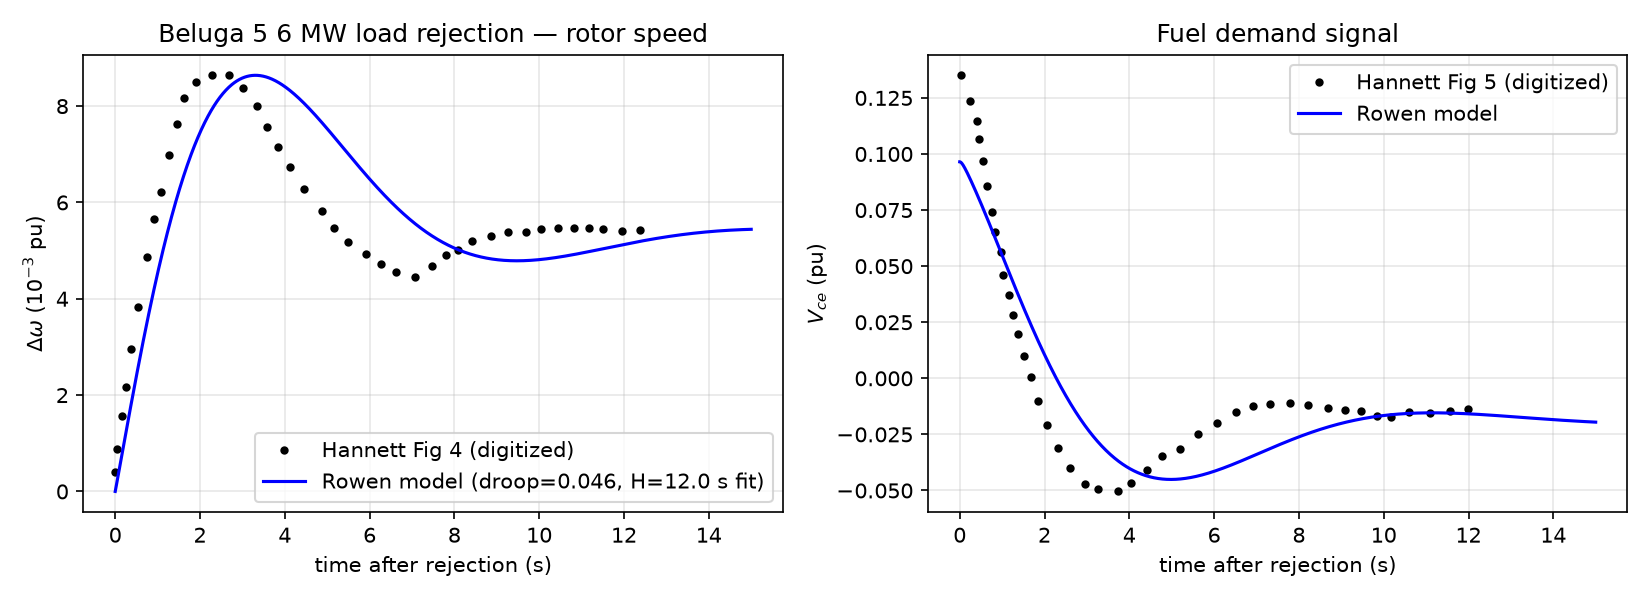
\includegraphics[width=\textwidth]{figs/hannett_overlay.png}
\caption{Beluga 5 6\,MW load rejection: model (line) vs.\ digitized
recordings (dots) from Hannett \& Khan (1993) Figs.~4/5. Left: rotor speed
deviation. Right: fuel demand signal $V_{ce}$. Droop and $H$ fit; the
$V_{ce}$ panel is an untuned prediction.}
\label{fig:hannett}
\end{figure}

\subsection{Thermodynamic validation}
First-law closure, $\dot m_f\,\text{LHV} = P + \dot m_\text{exh}
c_p (T_\text{exh} - T_\text{amb}) + \text{losses}$, with $c_p$ bracketed
$[1005, 1150]$\,J/kg/K (\texttt{pixi run vv-thermo}):

\begin{table}[h]\centering
\small
\begin{tabular}{lccccc}
\toprule
load & 0.2 & 0.4 & 0.6 & 0.8 & 1.0 \\
\midrule
Frame GT 235\,MW residual (\%) & $+17..{+}26$ & $+3..{+}11$ & $-2..{+}7$ & $-4..{+}4$ & $-6..{+}3$ \\
LM9000 SC residual (\%) & $+25..{+}32$ & $+17..{+}24$ & $+12..{+}19$ & $+10..{+}16$ & $+8..{+}14$ \\
\bottomrule
\end{tabular}
\caption{Unaccounted energy fraction (mechanical/generator/radiation
losses plus model error). The first law is never violated ($<0$ beyond
the $c_p$ bracket). The frame GT closes within the $c_p$ uncertainty at
load $\ge 0.4$. The LM9000's larger residual quantifies its documented
limitation: exhaust flow is derived from a \emph{fixed} air-fuel ratio, so
part-load exhaust energy is understated (real machines hold airflow much
flatter than fuel).}
\end{table}

Combined-cycle efficiencies are monotone and physical (heavy CCPP
26.1\,\%$\to$57.1\,\%; LM9000 CC 32.9\,\%$\to$50.5\,\%, design point
72.471\,MW/50.49\,\% preserved to 0.02\,\%). CO$_2$ factors sit between
stoichiometric CH$_4$ (2.743) and the EPA pipeline factor
($\approx$2.625).

\begin{table}[h]\centering
\small
\begin{tabular}{lccccc}
\toprule
LHV heat rate (kJ/kWh) at load: & 0.2 & 0.4 & 0.6 & 0.8 & 1.0 \\
\midrule
Frame GT 235\,MW (ThermoPower) & 21{,}658 & 13{,}063 & 10{,}807 & 9{,}729 & 9{,}083 \\
Heavy CCPP 338.7\,MW          & 13{,}806 &  8{,}617 &  6{,}999 & 6{,}574 & 6{,}301 \\
LM9000 simple cycle           & 16{,}397 & 11{,}842 & 10{,}324 & 9{,}565 & 9{,}109 \\
LM9000 combined cycle         & 10{,}933 &  8{,}702 &  7{,}853 & 7{,}406 & 7{,}130 \\
\bottomrule
\end{tabular}
\caption{Part-load heat rates from the post-fix models. Full-load values
sit in the expected class ranges (F-class SC $\sim$9{,}100; modern 1$\times$1
CC $\sim$6{,}300; aero SC $\sim$9{,}100; aero CC 7{,}130 = the LM9000
datasheet's 7{,}132 to 0.03\,\%).}
\end{table}

\subsection{Frozen regression baselines (Phase 4)}
The post-fix behavior is pinned by the automated suite so it cannot drift
silently:
\begin{table}[h]\centering
\small
\begin{tabular}{lll}
\toprule
scenario & metric & pinned value \\
\midrule
GGOV1, 11.5$\to$13.8\,MW step & nadir / final & 59.450 / 59.758\,Hz \\
TGOV1, 15$\to$18\,MW step & nadir / final & 59.300 / 59.701\,Hz \\
Two-mass, 15$\to$18\,MW step & nadir & 58.772\,Hz \\
GGOV1 at 15\,MW steady & fuel & 0.9290\,kg/s \\
Load17 replay (first 10\,min, $\times$10\,MW) & $|\Delta f|_{max}$ / fuel & 228.3\,mHz / 640.1\,kg \\
\bottomrule
\end{tabular}
\caption{Regression pins in \texttt{tests/test\_dynamics.py}. These
supersede the historical tier-table numbers, which were produced by the
pre-fix code (mixed bases, double damping, biased fuel mapping). Note the
two-mass nadir is deeper than the single-mass models' --- the spool-up lag
delays power delivery --- but its magnitude is qualitative until the
coupling law is calibrated (\S\ref{sec:multishaft}).}
\end{table}

\subsection{ANDES islanded case, v2}
The electrical-side case builder was upgraded (GENROU 6th-order machine
with an EXST1 exciter actually attached; $S_n = P_\text{rated}/0.85$;
governor limit at the turbine rating; and a reclose \emph{guard}: the
resync event is refused unless explicitly forced, because no sync-check
relay is modeled and an out-of-phase reclosure of an island is a
catastrophic event in reality). Five tests pin the ANDES interface facts
numerically, including one newly discovered: ANDES converts governor
power limits to the \emph{system} base at setup
($\texttt{VMAX.v} = V^{max} S_n / S_\text{sys}$).

%=====================================================================
\section{Constants: what is defensible and what is not}
%=====================================================================

The dossier (\texttt{docs/constants.md}) classifies every number. The
short version a reviewer should hear first:
\begin{itemize}[nosep]
\item \textbf{Pinned}: all GGOV1 block parameters (PES-TR-1 Appendix C,
  transcription verified value-by-value); NGG idle/full speeds (Pocket
  Guide); LHV; CO$_2$ factors; droop convention.
\item \textbf{Estimated}: $T_{act} = 0.15$\,s (electronic vs.\ hydraulic
  actuator argument); $\eta_\text{design} = 0.365$ (literature range
  35--38\,\%, NAVEDTRA cross-check); $S_n = 23$\,MVA / $T_\text{rate} =
  22$\,MW (site convention; the Pocket Guide's 26{,}250\,BHP
  $\approx$19.6\,MW \emph{shaft} figure for the Navy variant is a
  documented tension); Willans $b = 0.2$.
\item \textbf{Placeholder} (must not be presented as machine-specific):
  $H = 2.8$\,s (\emph{the} most consequential unpinned number --- nadir
  $\propto 1/H$; publish sensitivity over $H \in [1.5, 3.5]$\,s until a
  vendor WR$^2$ arrives); the Tier C coupling law and inertia split; the
  entire Tier E shaft/material/S--N set; $c_p$ of flue gas (two values in
  sibling modules).
\end{itemize}

%=====================================================================
\section{Limitations and recommended next steps}
%=====================================================================
\begin{enumerate}[nosep]
\item Pin $H$ (vendor WR$^2$ or an inertia test); until then quote nadir
  sensitivity.
\item Archive the LM9000 datasheet PDF and the LM2500 gen-set heat-rate
  sheet (upgrades two \textsc{estimated} anchors to \textsc{pinned}).
\item Retune $K_{pgov}/K_{igov}$ against vendor step data --- Hannett's
  field-derived governors are 2--4$\times$ hotter than PES-TR1 typicals,
  and the 2.32\,s vs.\ 1.14\,s gap in Table~3 is exactly this effect.
\item Calibrate the Tier C spool coupling to a recorded NGG acceleration.
\item Decide droop vs.\ isochronous for the islanded use case
  (\texttt{rselect} 1 vs.\ 0; both now implemented and verified) ---
  an open user decision.
\item The Tier E fatigue model needs shaft drawings and S--N data before
  any absolute life claim; today it is a screening tool.
\item Voltage dynamics: the scipy path holds $V = 1\pu$; studies of motor
  starts, faults, or reactive events must use the ANDES v2 case.
\end{enumerate}

%=====================================================================
\appendix
\section{Defect log from the pre-V\&V review (abridged)}
\label{app:defects}

Full text in \texttt{docs/vv\_log.md} Part 1. All fixed in Phase 0 and
covered by tests.
\begin{description}[nosep]
\item[G1 (per-unit bases)] GGOV1 ran on the generator base with a
  hand-edited valve limit. Consequences: three inconsistent ``thermal
  limits'' (26.1, 23, 22\,MW), an initial-load guard that admitted
  34.7\,MW, and tier-to-tier reinterpretation of $V^{min}$. Fix:
  turbine-base governor per PES-TR1 \S3.3 with the single $k_b$
  conversion.
\item[G2 (fuel mapping)] The fuel-valve signal (where 0.2 = zero power)
  was fed to a surrogate expecting a power fraction --- double-counting
  no-load fuel and biasing all fuel/CO$_2$ totals. Fix: native
  calibration \S\ref{sec:fuel}.
\item[G3 ($D_m$ sign)] Turbine ``damping'' injected energy on overspeed.
  Latent (default 0) but armed.
\item[G4 (structure)] \texttt{rselect} advertised but not implemented;
  TGOV1 limiter misplaced with a spurious extra pole; temperature path
  fed by back-derived power instead of fuel flow; reported $P_e$
  inconsistent with the $P_e$ actually simulated.
\item[G5 (damping double-count)] Machine $D=1$ \emph{and} load
  $\alpha=1.5$ simultaneously.
\item[P1 (LM9000 efficiency)] Part-load efficiency nearly flat (39.0\,\%
  at half load) --- replaced by the Willans line.
\item[P4 (citations)] A bottoming-cycle derate form mis-attributed to
  PES-TR1/CIGRE-238 --- retracted.
\item[Process] An unedited LLM chat transcript lived in \texttt{docs/} as
  apparent reference material --- quarantined with a provenance warning.
\end{description}

\section{Reproducing every number in this report}
\begin{verbatim}
cd DataCenter
pixi run vv-all        # 36 tests + smoke + ANDES cross-check
                       # + small-signal + Hannett + thermo
\end{verbatim}
Individual pieces: \texttt{pixi run test}, \texttt{vv-crosscheck},
\texttt{vv-smallsignal}, \texttt{vv-hannett}, \texttt{vv-thermo}.

\begin{thebibliography}{9}
\bibitem{pestr1} IEEE PES Task Force on Turbine-Governor Modeling,
``Dynamic Models for Turbine-Governors in Power System Studies,''
Technical Report PES-TR1, Jan.\ 2013. (Appendix C transcription vendored
in \texttt{papers/}.)
\bibitem{hannett} L.~N. Hannett and A.~Khan, ``Combustion turbine dynamic
model validation from tests,'' \emph{IEEE Trans.\ Power Systems},
vol.~8, no.~1, pp.~152--158, 1993.
\bibitem{rowen} W.~I. Rowen, ``Simplified mathematical representations of
heavy-duty gas turbines,'' \emph{ASME J.\ Eng.\ Power}, 105(4), 1983.
\bibitem{kundur} P.~Kundur, \emph{Power System Stability and Control},
McGraw-Hill, 1994 (\S11.1.4 for load damping).
\bibitem{yee} S.~K. Yee, J.~V. Milanovi\'c, and F.~M. Hughes, ``Overview
and comparative analysis of gas turbine models for system stability
studies,'' \emph{IEEE Trans.\ Power Systems}, 23(1), 2008.
\bibitem{cigre} CIGRE Task Force 38.02.25, ``Modeling of Gas Turbines and
Steam Turbines in Combined-Cycle Power Plants,'' Technical Brochure 238,
2003.
\end{thebibliography}

\end{document}
